% Beamer Presentation and Lecture Note Template
% Version 0.1
% by Paul Vesey

\mode<presentation> {
\usetheme{Antibes}
\setbeamercovered{invisible}
\setbeamertemplate{footline}[frame number]
\setbeamertemplate{navigation symbols}{} 
}

\usepackage{eurosym}
\usepackage{graphicx}
\usepackage{wasysym}
\usepackage{hyperref}
\usepackage{amsmath}
\usepackage{amssymb}
\usepackage{mathtools}
\usepackage{tikz}
\usepackage{pgf}
\usepackage{pgfplots}
\usepackage{pxfonts}
\usepackage{textcomp}
\usepackage{verbatim}
\usepackage{color}
\usepackage{xcolor}
\usepackage{fix-cm}


\author{Paul Vesey}
\institute[TUS]
{
Technological University of the Shannon \\
\medskip
{\emph{paul.vesey@tus.ie}}
}
\date{Autumn 2022}




\title[Project Management \& BIM]{Project Communications Management}



\begin{document}
%
\usetikzlibrary{arrows}
\usepgflibrary{patterns}

\tableofcontents
\newpage



\begin{frame}
\titlepage
\end{frame}\begin{center}\line(1,0){250}\end{center}
%
%


\section{Project Communications Management}

\subsection{Lecture 1}





\begin{frame}
\frametitle{Project Communications Management}
Project Management - Year 4\\
\textit{If you have to choose to believe the paperwork, you have already chosen wrongly.}\\
\end{frame}\begin{center}\line(1,0){250}\end{center}


\begin{frame}
\frametitle{Project Communications Management}
\begin{itemize}
	\item Project Communications Management involves the processes required to ensure timely and appropriate generation, collection, distribution, storage, retrieval, and ultimate disposition of project information.
	\item The processes provide the critical links among people and information that are necessary for successful communications.
\end{itemize}
\end{frame}\begin{center}\line(1,0){250}\end{center}


\begin{frame}
\frametitle{Plan Communications}
\textbf{Part of the Planning Process Group}
\begin{figure}
	\centering
		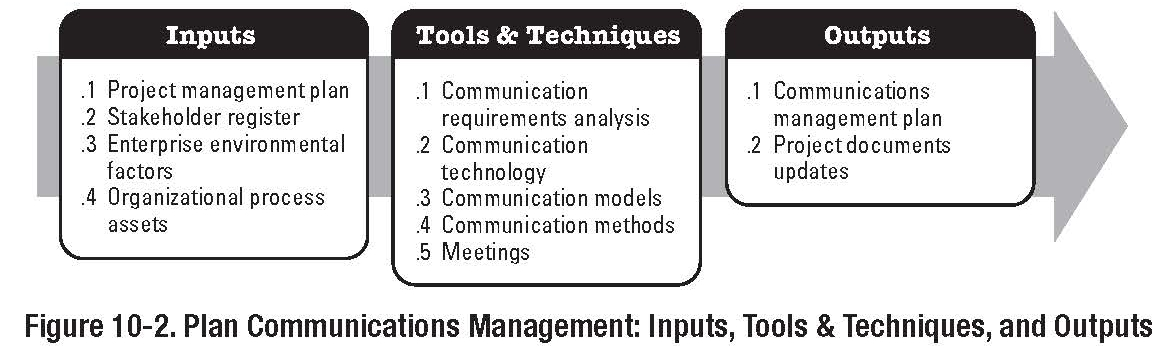
\includegraphics[width = 10cm]{images/Fig10-2.jpg}
	\label{fig:10-2}
\end{figure}
\end{frame}\begin{center}\line(1,0){250}\end{center}



\begin{frame}
\frametitle{Plan Communications \hfill\hfill Inputs}
\textbf{Communications Technology:} - Technology Factors:\\ 
\begin{itemize}
	\item Urgency of the need of information
	\item Availability of Technology: Broadband / HSDPA for site office
	\item Expected Project Staffing: 
		\begin{itemize}
			\item Site office with 2 persons v. 8 persons
		 	\item PABX, LAN, WAN, etc
		 	\item Do people know how to use the communication systems or will they have to be trained?
		\end{itemize}
	\item Length of Project
		\begin{itemize}
			\item 8 persons in office for 2 weeks v. 8 persons for 18 months
			\item Will technology change over the course of the project?
		\end{itemize}
	\item Project Environment: Face to Face or Virtual Environment?
\end{itemize}
\end{frame}\begin{center}\line(1,0){250}\end{center}

HSDPA: High-Speed Downlink Packet Access 
PABX: Private Automatic Branch Exchange
PSTN: Public Switched Telephone Network
LAN: Local Area Network
WAN: Wide Area Network
ISDN: Integrated Services Digital Network
VPN: Virtual Private Network



\begin{frame}
\frametitle{Plan Communications \hfill\hfill Inputs}
\textbf{Communication Methods}
\begin{itemize}
	\item Interactive Communications
		\begin{itemize}
			\item Web 2.0 Applications, Meetings, Skype, etc. 
		\end{itemize}
	\item Push Communications
		\begin{itemize}
			\item Letters, Memo, Reports, etc.
			\item No Guarantee that recipient has received or understood the message.
			\item Always ask for `read receipt' or `acknowledgment'
		\end{itemize}
	\item Pull Communications
		\begin{itemize}
			\item Information repositories, such as Moodle, shared drives, etc.
			\item User selects the information relevant to them.
			\item Requires considerable levels of control.
			\item Communication Models
		\end{itemize}
\end{itemize}
\end{frame}\begin{center}\line(1,0){250}\end{center}

Web 2.0 is a term used to describe interactive web applications.  In the early days of the Internet information was posted on static websites.  Users simply read information on-screen.  It was generally a one way process, feedback was generally by email.  As technologies progressed, users were then given the opportunity to post information directly on web pages etc.  This was the beginning of Web 2.0; i.e. interactive web applications such as blogging sites, Facebook, etc.  The term Web 2.0 is beginning to disappear as interactive web becomes the norm.


\begin{frame}
\frametitle{Plan Communications \hfill\hfill Tools and Techniques}
\textbf{Communication Requirements Analysis}\\
Requirements are defined by combining the type and format of information needed with an analysis of the value of that information, for instance technical information;
\begin{itemize}
	\item Format: drawing, specification, or both?
	\item Value: Drawing of Air Handler is vital for installation; performance specification is vital for purchase
\end{itemize}
Project Resources should only be used on communications that contribute to project success or where lack of communications lead to project failure
\end{frame}\begin{center}\line(1,0){250}\end{center}


\begin{frame}
\frametitle{Plan Communications \hfill\hfill Tools and Techniques}
\textbf{Communication Requirements Analysis}\\
Information required to determine project communications requirements typically include:
\begin{itemize}
	\item Organisation Charts
	\item Project Organisation and Stakeholder Responsibility Relationships
	\item Disciplines, Departments, and specialties involved in the project
	\item Logistics of how many people will be involved in the project, and their location
	\item Internal Information needs
	\item External information needs
	\item Stakeholder Information
\end{itemize}
\end{frame}\begin{center}\line(1,0){250}\end{center}


\begin{frame}
\frametitle{Plan Communications \hfill\hfill Outputs}
\textbf{Communications Management Plan}
\begin{itemize}
	\item Stakeholder Communication Requirements
	\item Information to be communicated: Format, Content, level of detail
	\item Person Responsible for communicating information
	\item Person or Groups who will receive the information
	\item Methods or Technologies used: Paper, email, etc.
	\item Frequency of the communications: weekly; monthly
	\item Escalation requirements
	\item Method of updating and refining the communications plan as the project progresses
	\item Glossary 
	\begin{itemize}
		\item `CPM' - `Critical Path Method' or `Construction Project Manager'?
		\item `CPI' - `Consumer Price Index' or `Cost Performance Index'?
	\end{itemize}
\end{itemize}
\end{frame}\begin{center}\line(1,0){250}\end{center}

Surprisingly, a glossary is often necessary to put all project team members on the same footing.  NASA are well known for their TLAs (Three Letter Acronyms).  The problem is what TLA is being referred to at any one time.  The CPI and CPM examples illustrate this problem, even in this lecture series..


\begin{frame}
\frametitle{Plan Communications \hfill\hfill Outputs}
\textbf{Communications Management Plan}\\
includes details of: 
\begin{itemize}
	\item Site Meeting (PM team)
	\item Progress Meetings (Client Meeting)
	\item Drawing Specifications (AutoCAD layers, etc.)
	\item Software to be used
		\begin{itemize}
			\item MS Excel, Word, Powerpoint, AutoCAD 2014, MapInfo, etc.
			\item Backwards Compatibility may be an issue
		\end{itemize}
\end{itemize}
\end{frame}\begin{center}\line(1,0){250}\end{center}




\begin{frame}
\frametitle{Distribute Information} 
\textbf{Part of the Executing Process Group}
\begin{figure}
	\centering
		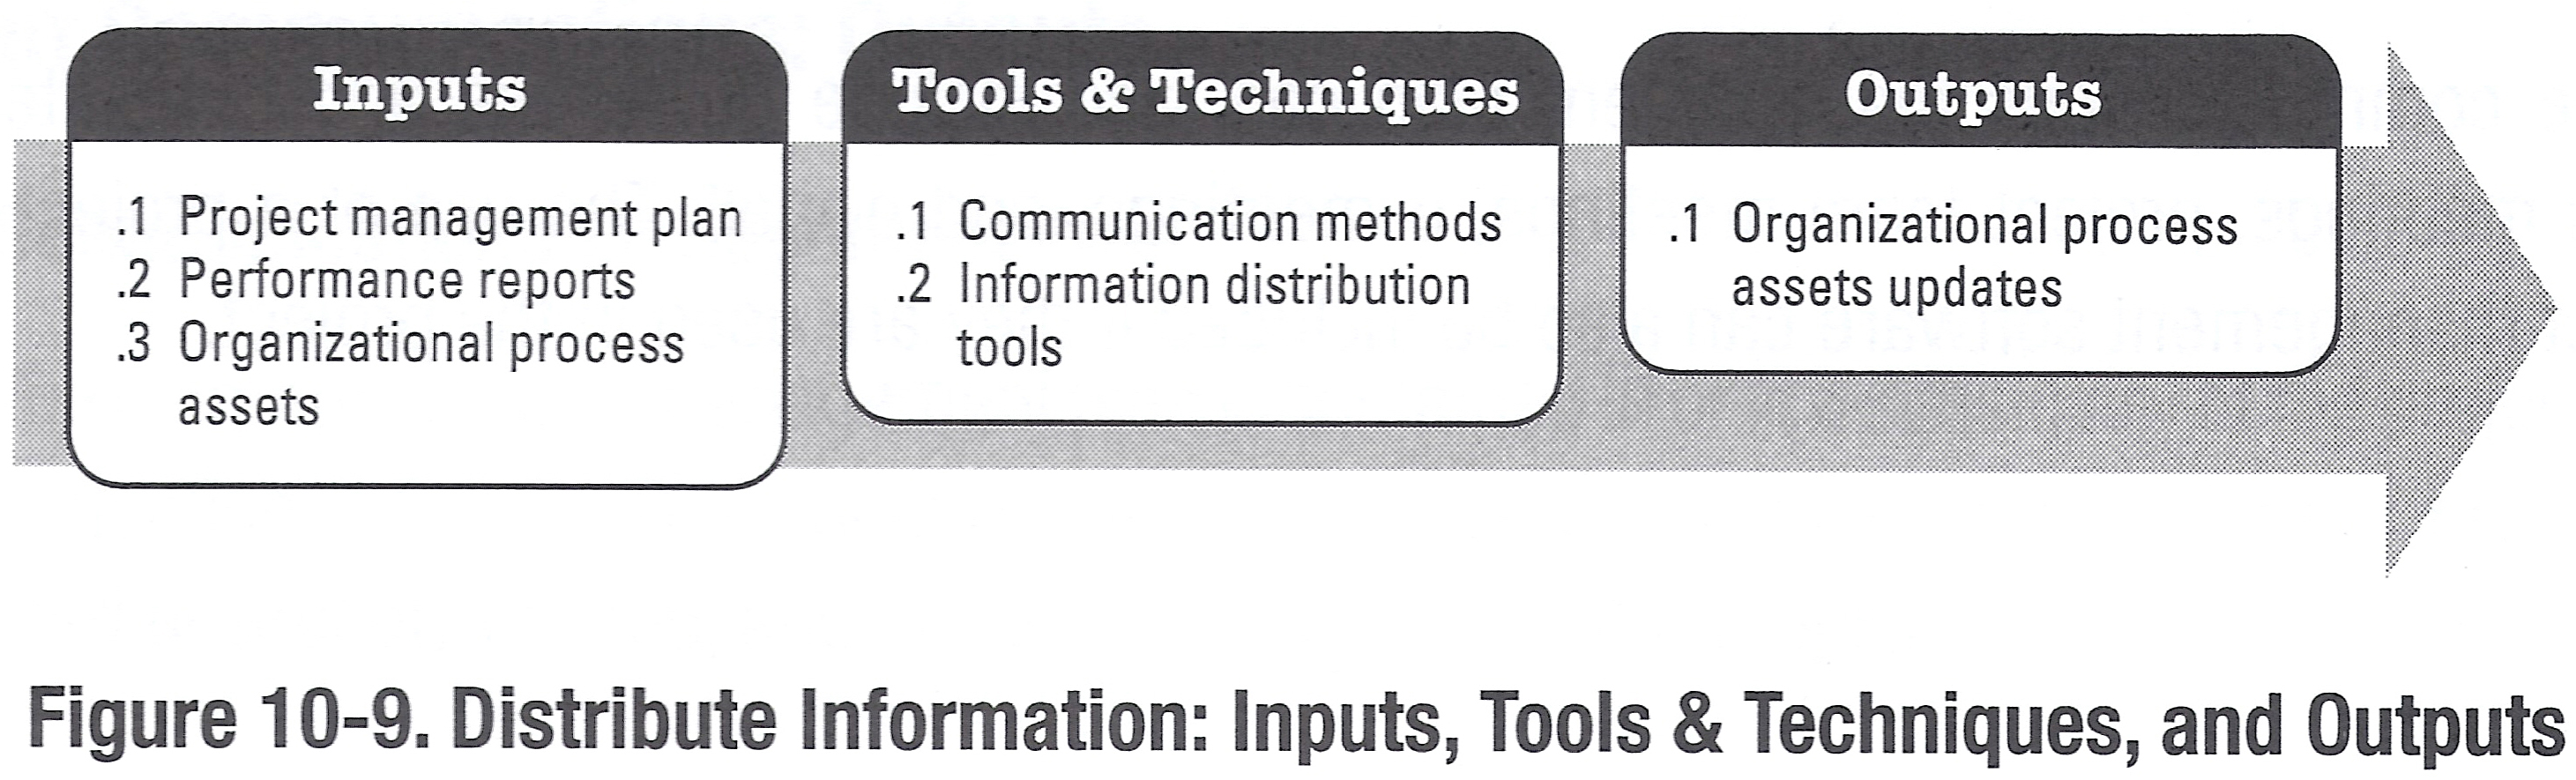
\includegraphics[width = 10cm]{images/Fig10-9.jpg}
	\label{fig:10-9}
\end{figure}
\end{frame}\begin{center}\line(1,0){250}\end{center}


\begin{frame}
\frametitle{Distribute Information}
\begin{itemize}
	\item Information Distribution involves making information available to project stakeholders in a timely manner.
	\item It includes implementing the communication management plan and responding to unexpected requests for information.
\end{itemize}
\end{frame}\begin{center}\line(1,0){250}\end{center}


\begin{frame}
\frametitle{Elements of Communications Theory}
\textbf{Sender Receiver Models}
\begin{itemize}
	\item Feedback Loops and barriers to communication
\end{itemize}
\textbf{Media Choice}
\begin{itemize}
	\item Verbal, Conversation; Presentation; etc.
\end{itemize}
\textbf{Written}
\begin{itemize}
	\item Memo (email); Report; Drawings; etc
\end{itemize}
\end{frame}\begin{center}\line(1,0){250}\end{center}



\begin{frame}
\frametitle{A model of communications}
\begin{figure}
	\centering
		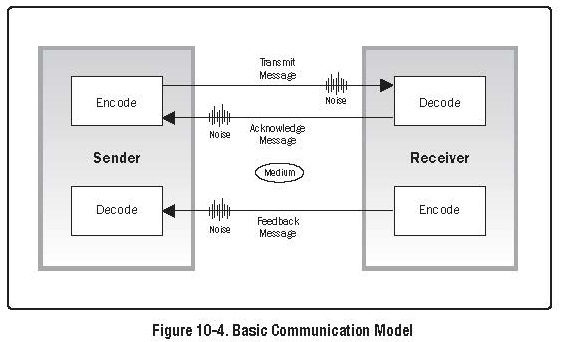
\includegraphics[width = 5cm]{images/Fig10-4.jpg}
	\label{fig:10-4}
\end{figure}
\begin{itemize}
	\item Encode - translation of thoughts or ideas onto language the is understood by others. 
	\item Message - the output of encoding.
	\item Medium - method used to convey the message.
	\item Noise - anything that interferes with the transmission and understanding of the message.
	\item Decode - translation of the message back into meaningful thoughts or ideas.
\end{itemize}
\end{frame}\begin{center}\line(1,0){250}\end{center}



\begin{frame}
\frametitle{Active v. Passive Voice \hfill\hfill Examples}
\begin{itemize}
	\item \textit{The project management plan \textbf{is intended} to facilitate key stakeholder involvement in the project (passive).}\\
	\item\textit{With our project management plan, \textbf{we intend} to obtain key stakeholder involvement. (active).}\\
	\item\textit{Reports \textbf{are written} in the third person impersonal (passive).}\\
	\item\textit{\textbf{Write reports} in third person impersonal (active).}
\end{itemize}	
	
\begin{itemize}
	\item This can run into conflict with 3rd person convention used in scientific and engineering communications.
\end{itemize}

\end{frame}\begin{center}\line(1,0){250}\end{center}




\begin{frame}
\frametitle{Active v. Passive Voice}  
\textbf{Characteristics of Passive Voice}
\begin{itemize}
	\item You can't assign responsibility.
	\item \textit{`Reports are written'} - this is an instruction from whom?
	\item Readers have to perform extra work to understand the sentence.
	\item Sentences tend to be longer.  
\end{itemize}
Can usually be identified by:
\begin{table}
	\scalebox{0.8}{
	\centering
		\begin{tabular}{|l|l|}
			\hline
				Word 	&	Example\\
			\hline
				is 		&	is dismissed\\
				are 	&	are completed\\
				was		&	was vacated\\
				were	&	were reversed\\
				been	&	been filed\\
				being	&	being confirmed\\
				be		&	be approved\\
				am 		&	am honoured\\
			\hline
		\end{tabular}
		}
\end{table}
\end{frame}\begin{center}\line(1,0){250}\end{center}


\begin{frame}
\frametitle{Distribute Information \hfill\hfill Inputs}
\textbf{Project Management Plan}\\
\textbf{Performance Reports}\\
\textbf{Organisational Process Assets}\\
\begin{itemize}
	\item Refer to Book
\end{itemize}
\end{frame}\begin{center}\line(1,0){250}\end{center}


\begin{frame}
\frametitle{Distribute Information \hfill\hfill Tools and Techniques}
\textbf{Communication Methods}\\
\textbf{Information Distribution Tools}\\
Note the importance of:\\
\begin{itemize}
	\item General communications skills
	\item Ensuring the right person gets the right information
	\item Ensuring that the receiver correctly interprets the information, i.e.FEEDBACK
	\item Lessons Learned Processes
	\begin{itemize}
		\item To capture communications (and project) methods that were successful or failed; and the reasons why.
		\item Not easy to achieve in the construction sector. Most PM team members in construction are involved in a number of projects, they may not always have the time to engage in a `project post-mortem'.
	\end{itemize}
\end{itemize}
\end{frame}\begin{center}\line(1,0){250}\end{center}


\begin{frame}
\frametitle{Distribute Information \hfill\hfill Tools and Techniques}
\textbf{Communication Methods}\\
\begin{itemize}
	\item Meetings, Document Distribution, Shared Access Databases, etc.
	\item Email, Fax, Voice, Video Conferencing, Web Conferencing, Skype, Google Hangouts 
\end{itemize}
\textbf{MS Project Enterprise Edition et. al.}\\
\textbf{Information Distribution Tools}\\
\begin{itemize}
	\item Tools to control the methods above.
	\item Note the importance of tracking who has received and needs to receive information.
	\item Speed and ease of use are vital to successful distribution systems.
\end{itemize}
\end{frame}\begin{center}\line(1,0){250}\end{center}




\begin{frame}
\frametitle{MapInfo Professional}
\begin{figure}
	\centering
		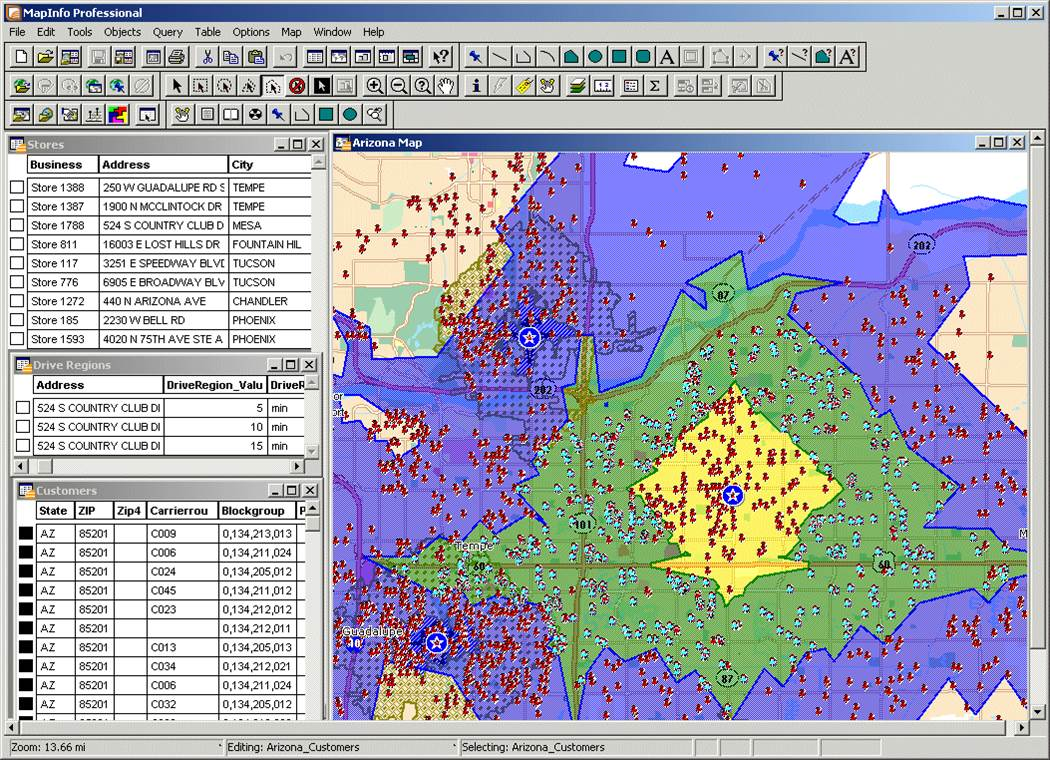
\includegraphics[width = 9cm]{images/mapinfo.jpg}
	\label{fig:mapinfo}
\end{figure}
\end{frame}\begin{center}\line(1,0){250}\end{center}

GIS systems are capable of showing highly complex spatial data.  However sometimes it is necessary to explain the function of diagrammatic objects and symbols.  Issues are also likely to emerge in relation to data transfer.  GIS systems tend to have proprietary file formats, making document interchange difficult.



\begin{frame}
\frametitle{Distribute Information \hfill\hfill Outputs}
\textbf{Organisational Process Assets Updates}
\begin{itemize}
	\item Stakeholder Notifications
	\item Project Reports
	\item Project Presentations
	\item Project Records
	\item Feedback from Stakeholders
	\item Lessons Learned Documentation
\end{itemize}
\textbf{Requested Changes (PMBOK 3rd Edition)}
\begin{itemize}
	\item Changes to the Information Distribution Process, which should be run through the Integrated Change Control Process
\end{itemize}
\end{frame}\begin{center}\line(1,0){250}\end{center}




%% END OF LECTURE SLIDE
\begin{frame}
\frametitle{Next Lecture \hfill\hfill Reading:}
`A Guide to the Project Management Body of Knowledge'\\ 
Chapter 10
\begin{figure}[h]
	\centering
		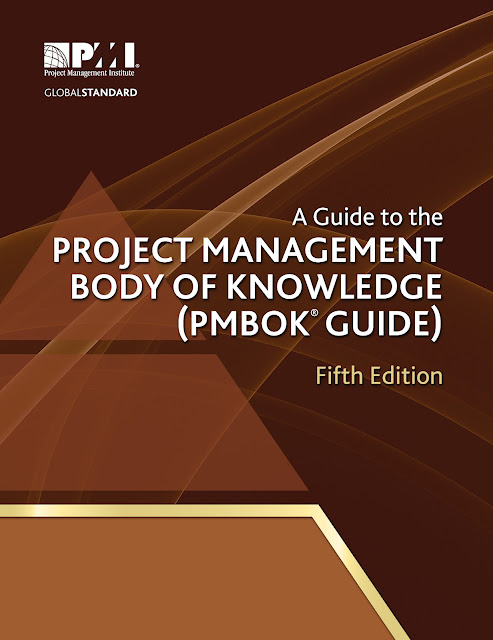
\includegraphics[width = 4cm]{images/book.jpg}
\end{figure}
\end{frame}\begin{center}\line(1,0){250}\end{center}
%% END OF LECTURE SLIDE


\subsection{Lecture 2}




\begin{frame}
\frametitle{Manage Stakeholder Expectations}
\textbf{Part of the Monitoring \& Controlling Process Group}
\begin{figure}
	\centering
		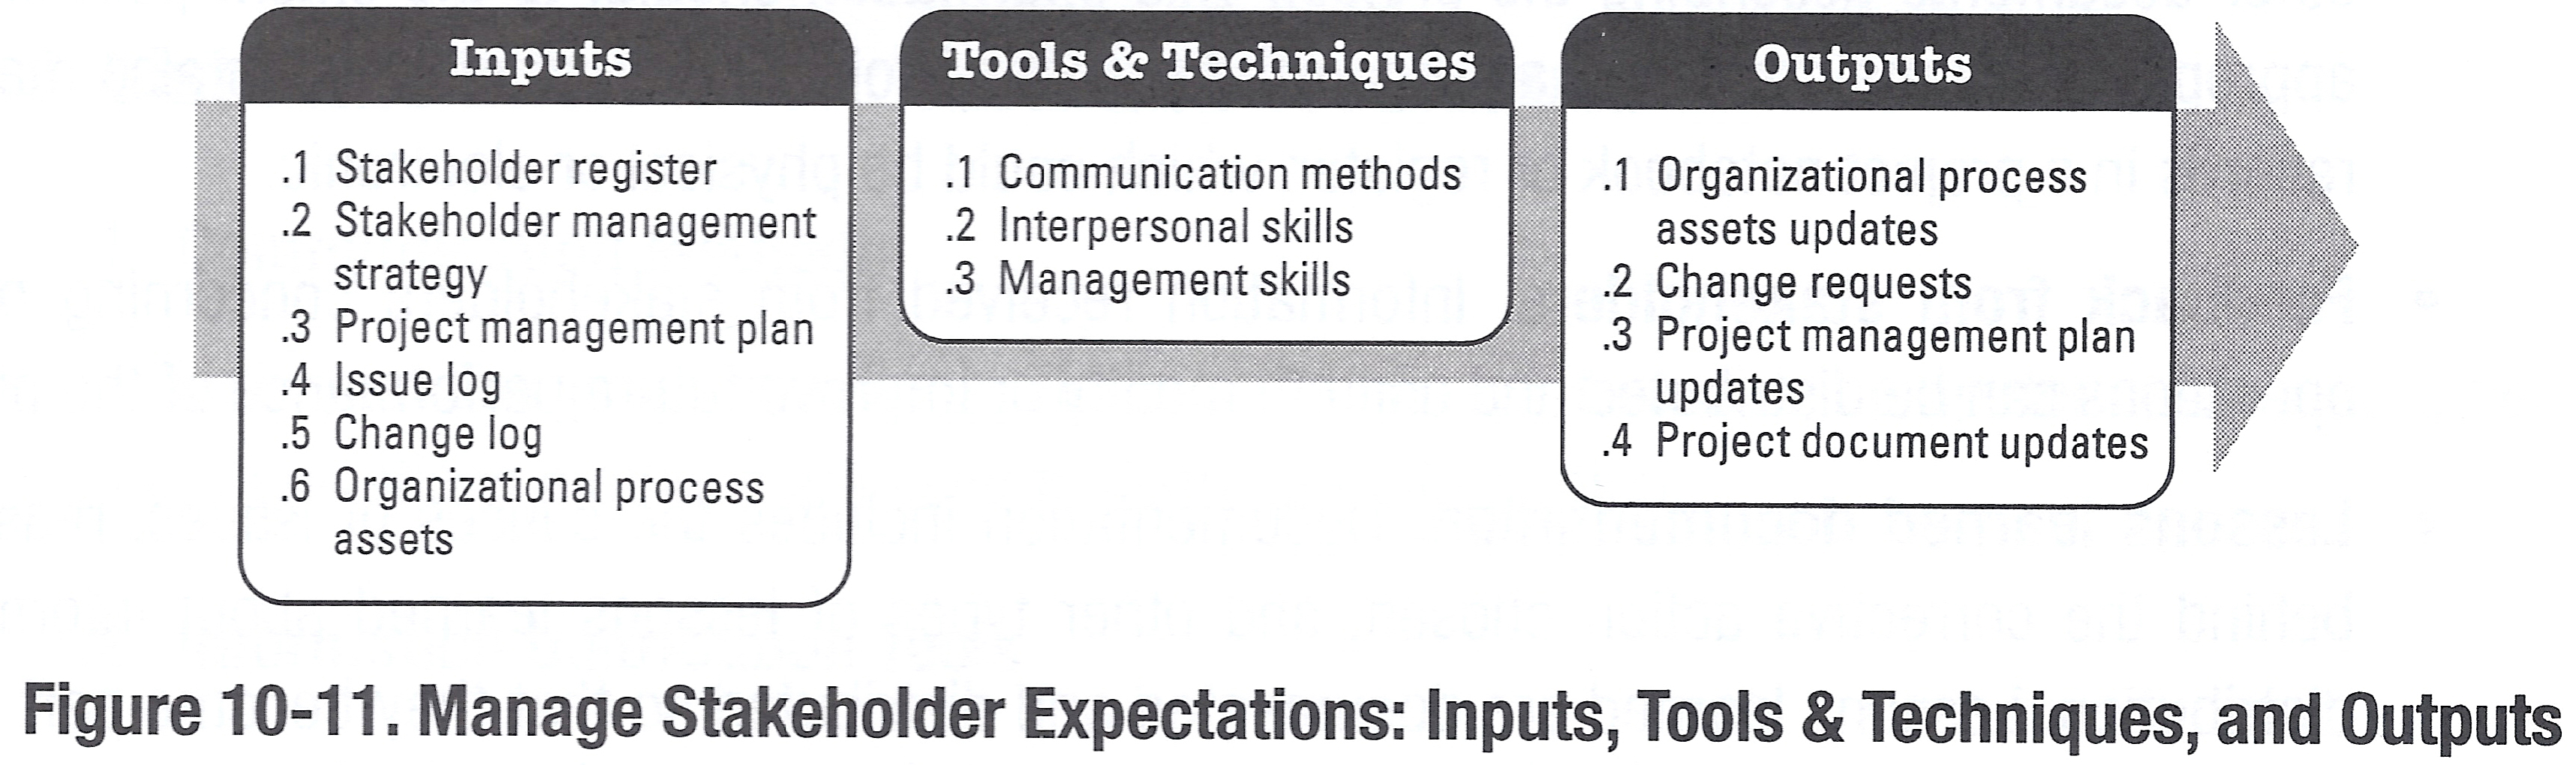
\includegraphics[width = 10cm]{images/Fig10-11.jpg}
	\label{fig:10-11}
\end{figure}
\end{frame}\begin{center}\line(1,0){250}\end{center}

\begin{frame}
\frametitle{Manage Stakeholders}
\begin{itemize}
	\item Managing Stakeholders refers to Managing Communications to satisfy the needs of, and resolve issues with, project stakeholders.
	\item Actively Managing Stakeholders increases the likelihood that the project will not veer off track due to unresolved issues.
	\item It also enhances the ability of persons to operate synergistically.
	\begin{itemize}
		\item The construction sector is notoriously adversarial.  Why?
	\end{itemize}
\end{itemize}
\end{frame}\begin{center}\line(1,0){250}\end{center}



\begin{frame}
\frametitle{Manage Stakeholder Expectations \hfill\hfill Inputs}
\textbf{Project Management Plan}\\
\textbf{Communications Management Plan}\\
\begin{itemize}
	\item Stakeholders communications needs and expectations are documented in the Communications Management Plan
\end{itemize}
\textbf{Organisational Process Assets}\\
\textbf{Issue Management Procedures}\\
\textbf{Change Control Procedures}\\
\textbf{Stakeholder Register}\\
\textbf{Stakeholder Management Strategy}\\
\textbf{Change Log}\\
\end{frame}\begin{center}\line(1,0){250}\end{center}


\begin{frame}
\frametitle{Manage Stakeholder Expectations \hfill\hfill Inputs}
\textbf{Issue Log}\\
\begin{itemize}
	\item Tool that can be used to document and monitor the resolution of issues
	\item An issue is clarified and stated in a way that it can be resolved.  An owner is assigned and a target date usually established for closure
	\item Unresolved Issues can become a major source of conflict
\end{itemize}
\begin{figure}
	\centering
		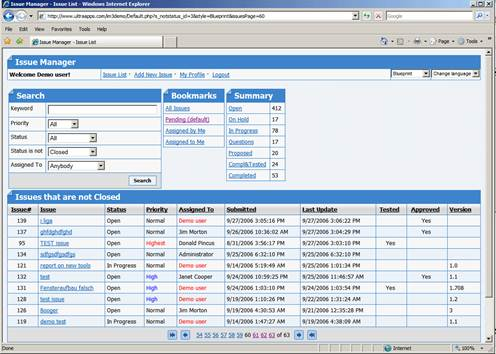
\includegraphics[width = 4cm]{images/issuemanager.jpg}
	\label{fig:issuemanager}
\end{figure}
\end{frame}\begin{center}\line(1,0){250}\end{center}




\begin{frame}
\frametitle{Manage Stakeholder Expectations \hfill\hfill Tools and Techniques}
\textbf{Communications Methods:}
\begin{itemize}
	\item Face to Face; Verbal
	\item Written; Reports etc.
	\item Mass Media; Billboards, Local and National Press, Radio, Web, etc.
\end{itemize}
\begin{figure}
	\centering
		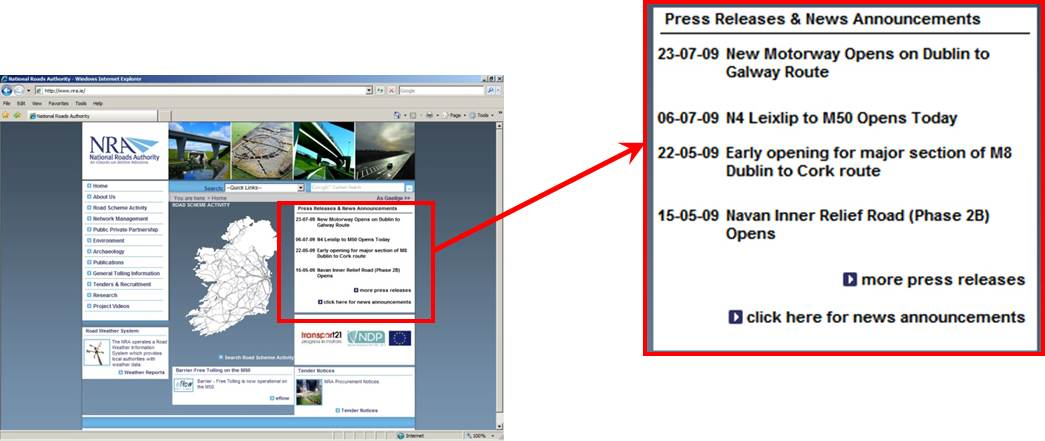
\includegraphics[width = 8cm]{images/nra.jpg}
	\label{fig:nra}
\end{figure}
\end{frame}\begin{center}\line(1,0){250}\end{center}



\begin{frame}
\frametitle{Manage Stakeholder Expectations \hfill\hfill Tools and Techniques}
\textbf{Interpersonal Skills}
\begin{itemize}
	\item Building Trust
	\item Resolving Conflict
	\item Overcoming Resistance to change
	\item Active Listening
\end{itemize}
\textbf{Management Skills}
\begin{itemize}
	\item Presentation Skills
	\item Negotiating 
	\item Writing
	\item Public Speaking
\end{itemize}
\end{frame}\begin{center}\line(1,0){250}\end{center}

Active listening is about confirming what the speaker has said by restating or paraphrasing a response.  In effect, is is about closing the communications loop. This can work well in small groups, but can become tiresome if overused.  In a lecture/presentation environment it is generally not encouraged; opportunities for feedback are generally left to the end.

\begin{frame}
\frametitle{Manage Stakeholder Expectations \hfill\hfill Outputs}
\textbf{Organisational Process Assets Updates}
\begin{itemize}
	\item Lessons Learned Documentation etc.
	\item Causes of Issues / Reasons for corrective actions taken
\end{itemize}
\textbf{Change Requests}\\
\textbf{Project Management Plan Updates}\\
\textbf{Project Document Updates}
\begin{itemize}
	\item Stakeholder Management Strategy
	\item Stakeholder Register
	\item Issue Log
\end{itemize}
\end{frame}\begin{center}\line(1,0){250}\end{center}



\begin{frame}
\frametitle{Report Performance}
\textbf{Part of the Monitoring \& Controlling Process Group}
\begin{figure}
	\centering
		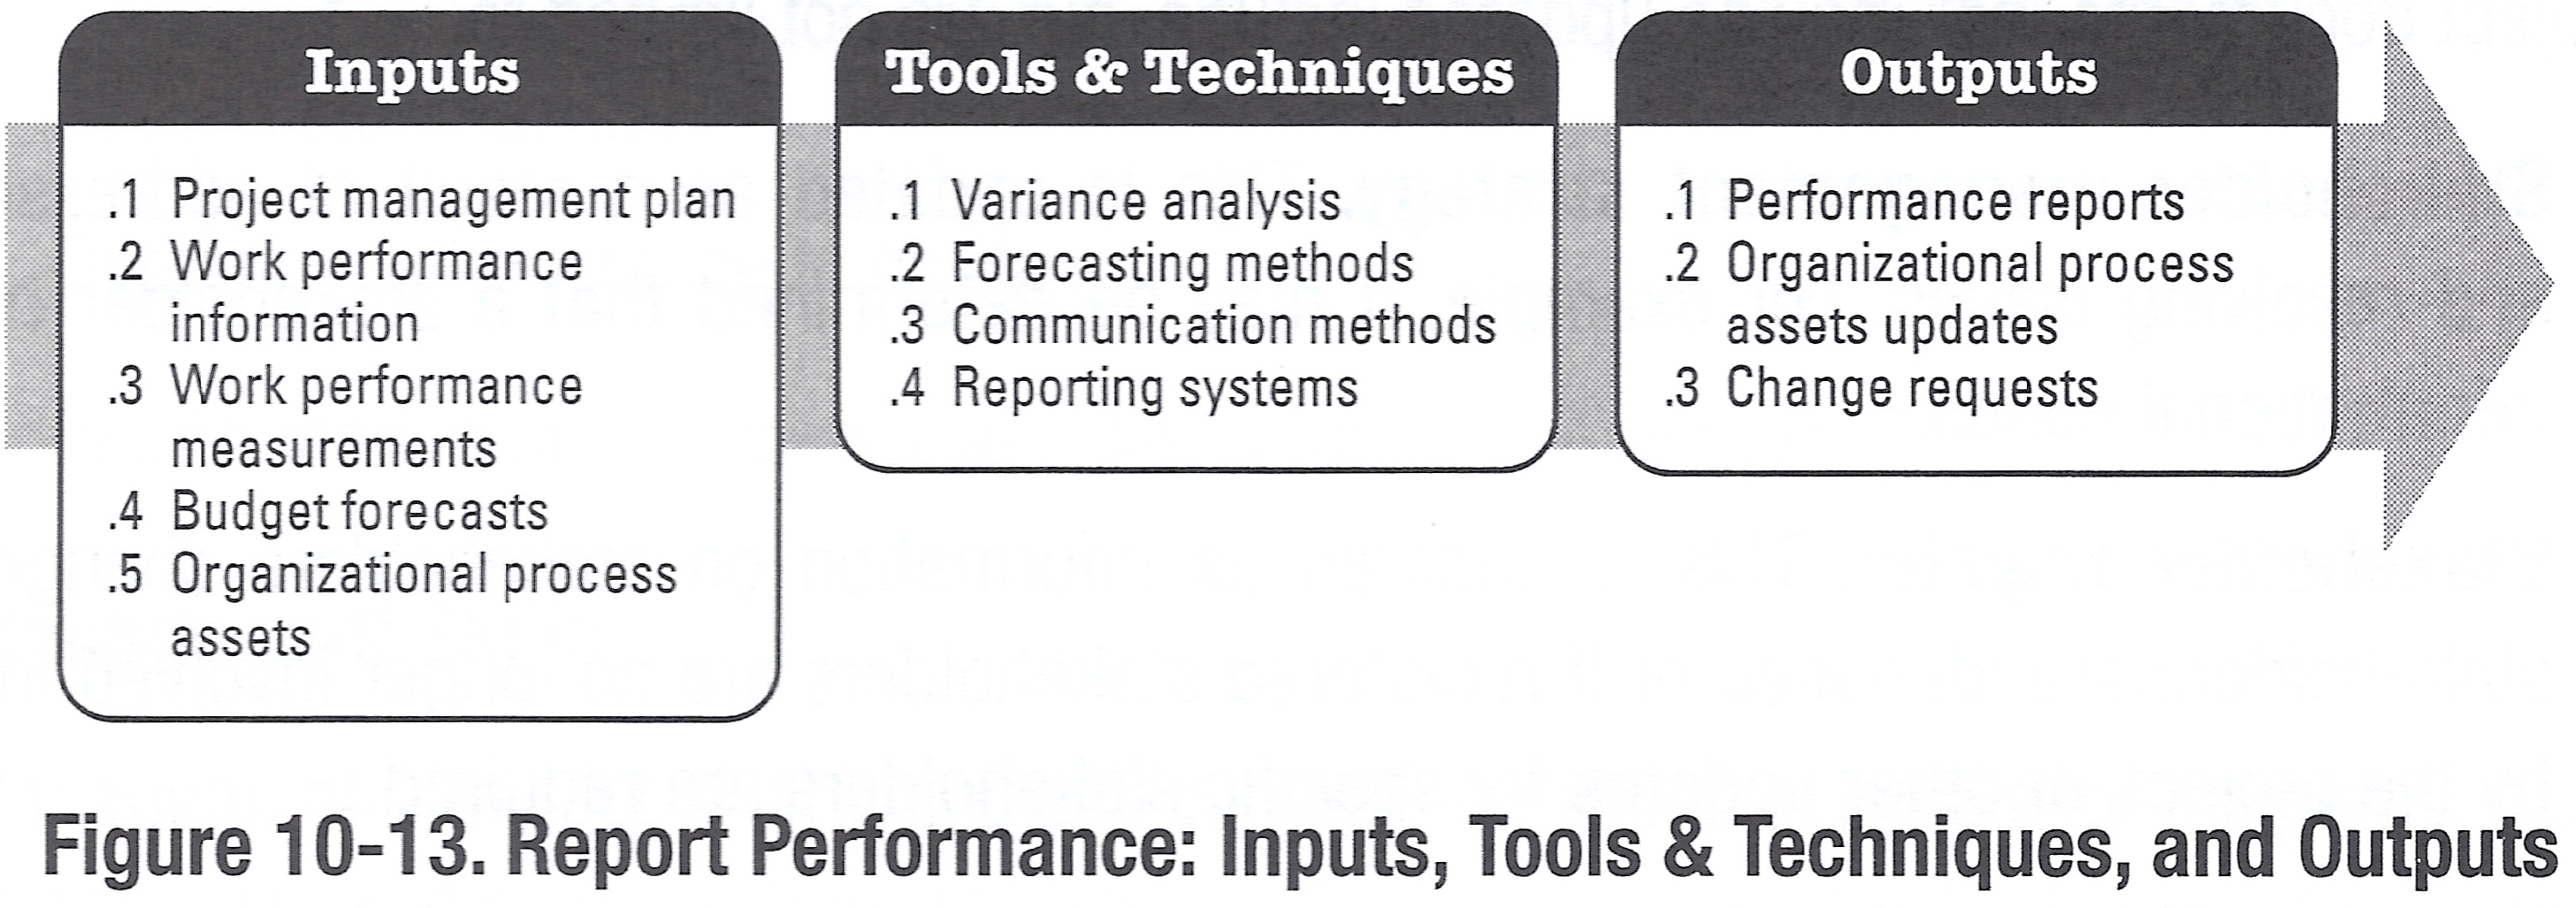
\includegraphics[width = 10cm]{images/Fig10-13.jpg}
	\label{fig:10-13}
\end{figure}
\end{frame}\begin{center}\line(1,0){250}\end{center}


\begin{frame}
\frametitle{Report Performance}
The Performance Reporting Process involves the collection of all baseline data, and distribution of performance information to stakeholders.  Performance Information includes data in relation to:
\begin{itemize}
	\item Scope
	\item Schedule
	\item Cost
	\item Quality
	\item Risk
	\item Procurement
	\item Etc.
\end{itemize}
\end{frame}\begin{center}\line(1,0){250}\end{center}


\begin{frame}
\frametitle{Report Performance \hfill\hfill Inputs}
\textbf{Project Management Plan}
		\begin{itemize}
			\item Performance Measurement Baseline
		\end{itemize}
\textbf{Work Performance Information}
		\begin{itemize}
			\item Completion Status of Deliverables
		\end{itemize}
\textbf{Work Performance Measurement}
		\begin{itemize}
			\item SV; SPI; CPI; etc.
		\end{itemize}
\textbf{Budget Forecasts}
		\begin{itemize}
			\item EAC; ETC; Trend Analysis  
		\end{itemize}
\textbf{PMBOK 3rd Edition  also included:}
	\begin{itemize}
		\item Quality Control Measures: Actual Quality Measurements
		\item WWTP Commissioning; BOD$_{5}$, Suspended Solids,  Nitrogen, Phosphorous
		\item Large Buildings: AHU performance; volumetric flow rates
		\item Approved Change Requests: Approved Changes to Project Scope
		\item Deliverables: Approval Status of Deliverables
	\end{itemize}
\end{frame}\begin{center}\line(1,0){250}\end{center}



\begin{frame}
\frametitle{Report Performance \hfill\hfill Tools \& Techniques}
\textbf{Variance Analysis}\\
\textbf{Forecasting Methods}
\begin{itemize}
	\item Time Series Methods: Historical Data used to predict future outcomes
	\item Causal/Econometric Methods: Cause and Effect used to predict future outcomes. It relies on determining the variables which will have the greatest effect on the outcome. 
\end{itemize}
\textbf{Judgmental Methods}
\begin{itemize}
	\item Intuitive Judgment, opinions and probabilities 
\end{itemize}
\textbf{Others}
\begin{itemize}
	\item Simulation, etc.
\end{itemize}
\end{frame}\begin{center}\line(1,0){250}\end{center}



\begin{frame}
\frametitle{Report Performance \hfill\hfill Tools \& Techniques}
\textbf{Communications Methods}
\begin{itemize}
	\item Status Review Meetings
\end{itemize}
\textbf{Reporting Systems}
\begin{itemize}
	\item Systems have to be designed and implemented to support the performance reporting.
\end{itemize}
\end{frame}\begin{center}\line(1,0){250}\end{center}


\begin{frame}
\frametitle{Report Performance \hfill\hfill Outputs}
\textbf{Performance Reports}
\begin{itemize}
	\item Summary and Presentation of the information gathered, and results of any analysis against baseline information, may include S-curves, EVM, etc.
	\item Current Status of Risks and Issues
	\item Work to be completed during the next reporting period
	\item Summary of changes approved in the reporting period
	\item Recommended Corrective Actions: actions required to bring the project back on schedule etc.
	\item Forecasts: Completion Forecasts based on performance information (EAC and ETC)
\end{itemize}
\textbf{Change Requests}
\begin{itemize}
	\item Performance analysis often generates change requests\dots
	\item These should be run through the Integrated Change Control Process
\end{itemize}
\textbf{Organisational Process Assets Updates}
\begin{itemize}
	\item Lessons Learned Documentation, etc.
\end{itemize}
\end{frame}\begin{center}\line(1,0){250}\end{center}



\begin{frame}
\frametitle{Report Performance}
\begin{figure}
	\centering
		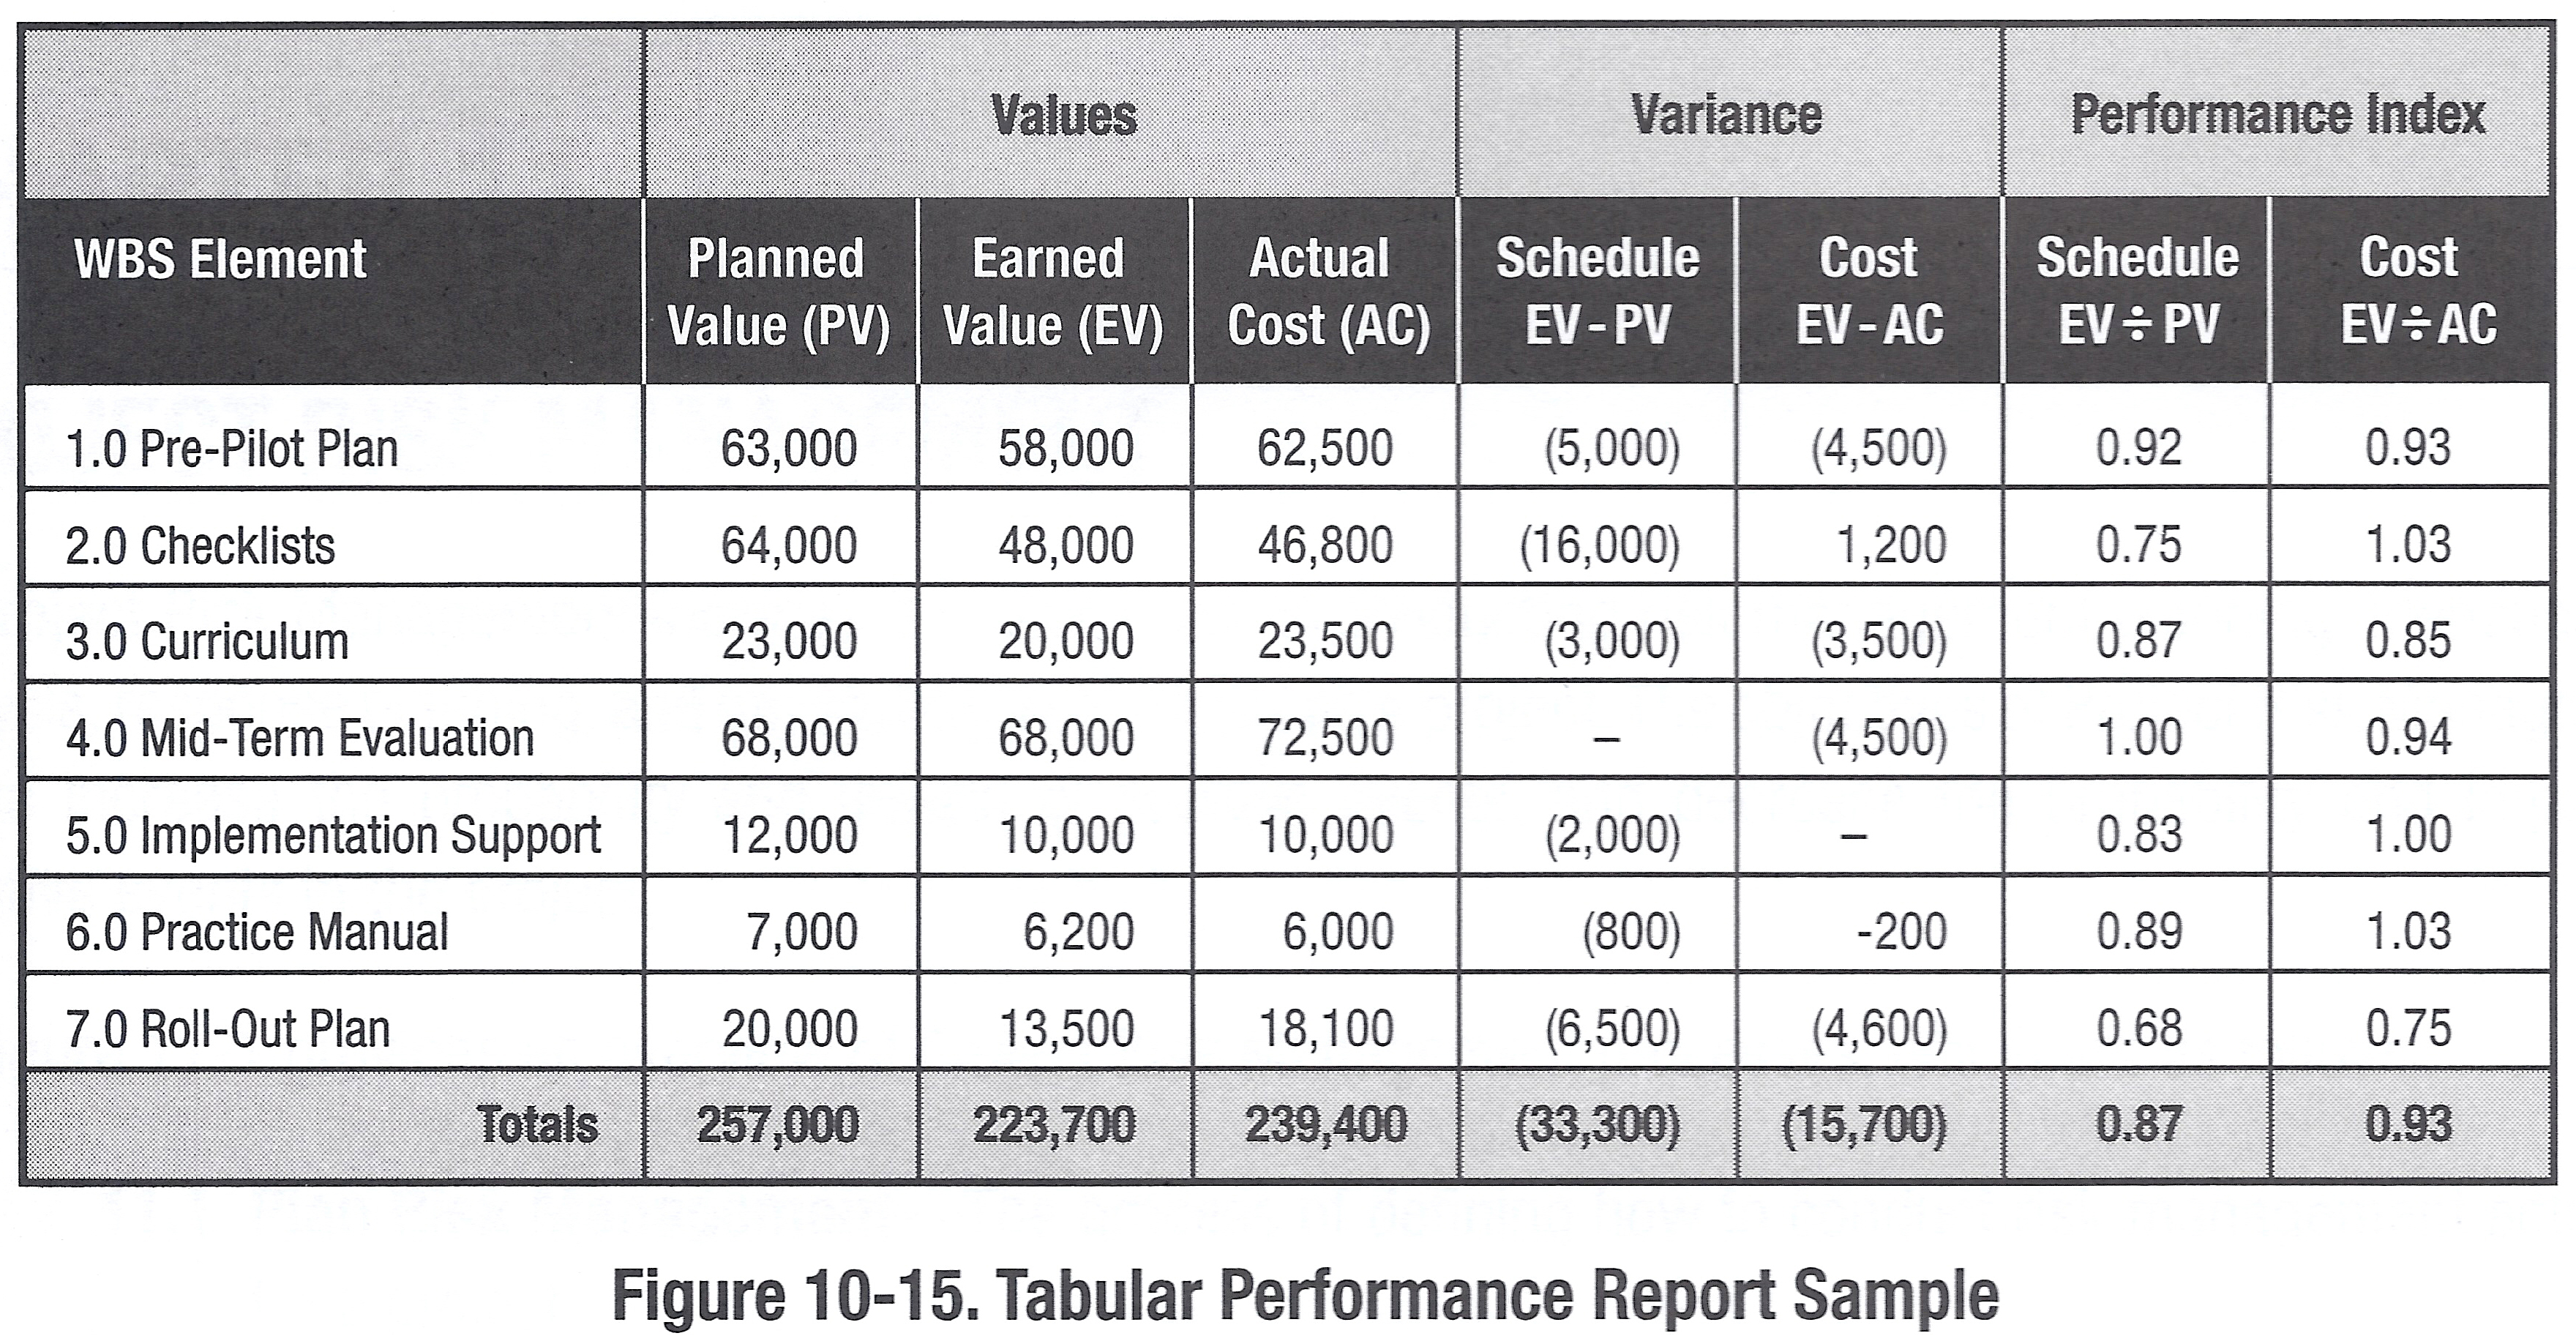
\includegraphics[width = 10cm]{images/Fig10-15.jpg}
	\label{fig:10-15}
\end{figure}
\end{frame}\begin{center}\line(1,0){250}\end{center}


%% END OF LECTURE SLIDE
\begin{frame}
\frametitle{Next Lecture \hfill\hfill Reading:}
`A Guide to the Project Management Body of Knowledge'\\ 
Chapter 4
\begin{figure}[h]
	\centering
		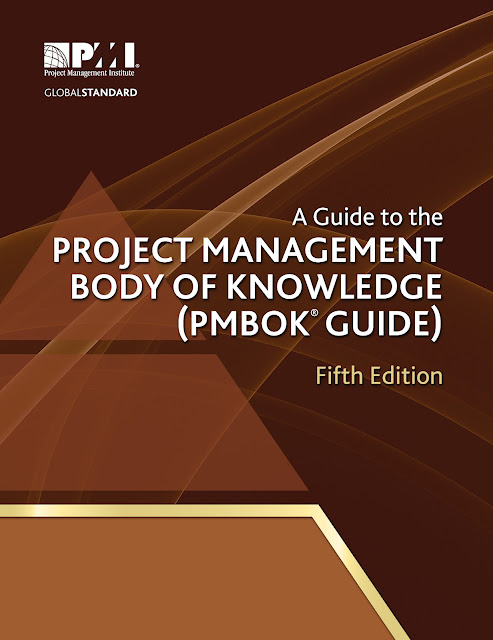
\includegraphics[width = 4cm]{images/book.jpg}
\end{figure}
\end{frame}\begin{center}\line(1,0){250}\end{center}
%% END OF LECTURE SLIDE




\end{document}
